%! Author = loreb
%! Date = 31/10/2023

% Preamble
\documentclass[11pt]{article}

% Packages
\usepackage{amsmath}
\usepackage{graphicx}
\usepackage{float}
\usepackage{csvsimple}
\usepackage{hyperref}
\usepackage{listings}
\usepackage{xcolor}
\usepackage{subcaption}
\usepackage{mdwtab}

\definecolor{codegreen}{rgb}{0,0.6,0}
\definecolor{codegray}{rgb}{0.5,0.5,0.5}
\definecolor{codepurple}{rgb}{0.58,0,0.82}
\definecolor{backcolour}{rgb}{0.95,0.95,0.92}

\lstdefinestyle{mystyle}{
    backgroundcolor=\color{backcolour},
    commentstyle=\color{codegreen},
    keywordstyle=\color{magenta},
    numberstyle=\tiny\color{codegray},
    stringstyle=\color{codepurple},
    basicstyle=\ttfamily\footnotesize,
    breakatwhitespace=false,
    breaklines=true,
    captionpos=b,
    keepspaces=true,
    numbers=left,
    numbersep=5pt,
    showspaces=false,
    showstringspaces=false,
    showtabs=false,
    tabsize=2
}
\lstset{style=mystyle}
\graphicspath{{../results/csv}}

\title{BloomFilter Speedup on setup and filter with Joblib}
\title{%
  Parallelizzazione di un BloomFilter per la classificazione di email di spam \\
  \large Parallel Programming for Machine Learning}
\author{Lorenzo Baiardi, Thomas Del Moro}
\date{GG MM AAAA}

% Document
\begin{document}

    \maketitle
    \clearpage

    \section{Introduzione}\label{sec:introduzione}
    Il nostro progetto si concentra sulla parallelizzazione di un BloomFilter impiegato per la classificazione di email considerate spam.
    Per raggiungere questo obiettivo, utilizziamo le librerie Omp e Joblib per implementare il parallelismo.

    Le fasi che intendiamo parallelizzare sono il setup iniziale e la fase di filtraggio.
    Vogliamo analizzare come lo speedup varia in relazione alle dimensioni dell'insieme di dati utilizzato per il training.
    Allo stesso modo, intendiamo valutare l'effetto dello speedup in funzione del numero di processi impiegati, delle dimensioni del dataset
    e delle diverse implementazioni utilizzate.

    \section{Analisi del problema}\label{sec:analisi-del-problema}
    Il BloomFilter rappresenta una struttura dati probabilistica finalizzata a determinare la presenza di un elemento all'interno di un insieme,
    nel contesto specifico, se una determinata email è considerata spam o meno.
    La fase iniziale di configurazione del BloomFilter coinvolge il calcolo delle funzioni hash e la creazione del vettore di bit.
    Quest'ultima operazione si basa sulla dimensione dell'insieme utilizzato per il training e sulla probabilità attesa di ottenere falsi positivi.
    La formula per il calcolo della dimensione del vettore di bit è la seguente:
    \begin{equation}
        size = -\frac{n \ln{p}}{(\ln{2})^2}\label{eq:dim_bit}
    \end{equation}
    Dove $size$ è la dimensione del vettore di bit per il training e $n$ è la dimensione dell'insieme che si vuole utilizzare.

    La formula per il calcolo del numero di funzioni hash è la seguente:
    \begin{equation}
        h = \frac{size}{n} \ln{2}\label{eq:num_hash}
    \end{equation}
    Dove $h$ è il numero di funzioni hash da utilizzare per il training.

    Dopo aver fornito al BloomFilter il dataset di training, quest'ultimo procede al calcolo delle $h$ funzioni hash per ciascuna email,
    impostando a 1 i bit nelle posizioni calcolate.
    Per determinare se un'email è classificata come spam o meno, il BloomFilter esegue nuovamente il calcolo delle $h$
    funzioni hash e verifica se i bit corrispondenti alle posizioni calcolate sono settati a 1.

    \section{Parallelizzazione}\label{sec:parallelizazzione}
    Il codice sequenziale di riferimento da parallelizzare per la fase di setup è il seguente, rispettivamente per la versione c++ e python:
\lstinputlisting[language=c++, firstline=22, lastline=28,label={lst:sequential-code-setup-omp}]{BloomFilter.cpp}
\lstinputlisting[language=python, firstline=33, lastline=39,label={lst:sequential-code-setup-joblib}]{../src/bloom_filter.py}

Nella fase sequenziale della configurazione, dopo un'iniziale fase di inizializzazione finalizzata al calcolo del valore
ottimale del vettore di bit e del numero di funzioni hash in base al valore di probabilità di falsi positivi,
si procede con l'indicizzazione nel vettore di bit per ciascuna email.

Il codice sequenziale di riferimento da parallelizzare per la fase di filter è il seguente, rispettivamente per la versione c++ e python:
\lstinputlisting[language=c++, firstline=54, lastline=60,label={lst:sequential-code-filter-omp}]{BloomFilter.cpp}
\lstinputlisting[language=python, firstline=58, lastline=66,label={lst:sequential-code-filter-joblib}]{../src/bloom_filter.py}

Nella fase sequenziale del processo di filtraggio, si inizializza una variabile di conteggio per i
falsi positivi, la quale sarà incrementata ogni volta che un'email viene identificata come spam.

\subsection{OpenMP}\label{subsec:omp}
OpenMP (Omp) è una libreria in linguaggio C progettata per consentire la parallelizzazione di funzioni e cicli for.
Nel contesto di questo lavoro, abbiamo adottato la funzione \texttt{omp parallel for} per parallelizzare le operazioni
di setup e filtraggio del BloomFilter.

Successivamente, abbiamo analizzato il tempo impiegato dalle funzioni di setup e filtraggio in relazione al numero
di processi utilizzati, confrontandolo con il tempo richiesto nella versione sequenziale.
\lstinputlisting[language=c++, firstline=30, lastline=47, label={lst:openmp-setup-code}]{BloomFilter.cpp}
Per la fase di setup, abbiamo parallelizzato l'indicizzazione nel vettore di bit per ogni email, utilizzando la direttiva \texttt{omp parallel for},
e la direttiva \texttt{omp critical} per garantire l'accesso esclusivo al vettore di bit, evitando così l'accesso concorrente.

Per quanto riguarda l'operazione di filtraggio, abbiamo ideato due diverse implementazioni.
\lstinputlisting[language=c++, firstline=62, lastline=74, label={lst:openmp-filter-code}]{BloomFilter.cpp}
La prima realizzazione prevede l'impiego della direttiva \texttt{omp parallel for} al fine di parallelizzare il processo
di verifica della presenza di un'email all'interno del BloomFilter.
In aggiunta, viene utilizzata la direttiva \texttt{omp atomic} per assicurare l'accesso esclusivo alla variabile
incrementale utilizzata per il conteggio dei falsi positivi.

\lstinputlisting[language=c++, firstline=76, lastline=90, label={lst:openmp-filter2-code}]{BloomFilter.cpp}
La seconda realizzazione, al contrario, impiega una variabile incrementale dedicata per ciascun thread, e la somma di
tali variabili al termine dell'operazione di filtraggio.
Inoltre, si fa uso della direttiva \texttt{omp atomic} per assicurare l'accesso esclusivo alla variabile
incrementale globale durante questa fase.
Verificheremo in seguito la differenza tra queste due implementazioni.

\subsection{Joblib}\label{subsec:joblib}
Joblib è una libreria Python ideata per abilitare la parallelizzazione di funzioni e cicli for.
La funzione \texttt{Parallel} prende come input sia il numero di processi da utilizzare che la funzione da parallelizzare.
Nell'ambito di questo studio, abbiamo sfruttato la funzione \texttt{Parallel} per parallelizzare sia le fasi di
preparazione (setup) che quelle di filtraggio del BloomFilter.

Successivamente, abbiamo analizzato il tempo richiesto dalle funzioni di setup e filtraggio in relazione al numero
di processi utilizzati, confrontandolo con il tempo necessario nella versione sequenziale.
\lstinputlisting[language=python, firstline=41, lastline=50,label={lst:joblib-code-setup}]{../src/bloom_filter.py}
Analogamente all'approccio con Omp, abbiamo parallelizzato l'indicizzazione nel vettore di bit per ciascuna email
mediante l'utilizzo della funzione \texttt{Parallel}, suddividendo il vettore di email in chunk corrispondenti al
numero di processi impiegati.
In aggiunta, il vettore di bit viene memorizzato in memoria attraverso l'utilizzo della funzione \texttt{memmap},
consentendo sia di condividerlo tra i vari processi che di conservare i risultati ottenuti in memoria.

\lstinputlisting[language=python, firstline=68, lastline=80,label={lst:joblib-code-filter}]{../src/bloom_filter.py}
Nella fase di filtraggio, abbiamo parallelizzato la verifica della presenza di un'email nel BloomFilter mediante
l'utilizzo della funzione \texttt{Parallel}.
Anche in questo caso, abbiamo diviso il vettore di email in chunk corrispondenti al numero di processi impiegati.

In seguito, abbiamo voluto esaminare l'impatto della dimensione del chunk anche al di là del numero di processi
utilizzati, al fine di valutare se un suo aumento potesse o meno offrire vantaggi in termini di tempo e di speedup.

    \section{Caratteristiche della macchina}\label{sec:caratteristiche-della-macchina}
    La macchina utilizzata per i test ha le seguenti caratteristiche:
    \begin{itemize}
        \item \textbf{CPU}: Intel Core i7-1360P (4 P-Core, 8 E-Core, 12 Cores, 16 Threads)
        \item \textbf{RAM}: 16GB
        \item \textbf{Sistema Operativo}: Windows 11
    \end{itemize}

    \section{Test}\label{sec:test}
I test sono stati condotti su un dataset composto da 10.000 fino a 10.000.000 di email, considerando probabilità di
falsi positivi pari a 0,10, 0,05 e 0,01.
Per una valutazione preliminare dei tempi di esecuzione, dello speedup e del False Positive Rate (FPR),
focalizziamo l'attenzione sul valore di 0,05 per il FPR\@.

Gli altri valori di FPR sono riportati nell'appendice~\ref{sec:fpr-001} e~\ref{sec:fpr-010}.

Il numero di processi considerati varia da 1 (modalità sequenziale) al massimo numero di processi disponibili sulla
macchina, ossia 16.
Le email sono state generate casualmente attraverso il generatore di email presente nel file \texttt{email\_generator.py}.
Poiché i test coprono un intervallo da 10.000 a 10.000.000 di email, il numero di funzioni hash è approssimativamente
pari a 5, e le dimensioni del vettore di bit variano da un minimo di 62.353 a un massimo di 62.352.243.

\subsection{OpenMP}\label{subsec:openmp-test}
\subsubsection{Setup}\label{subsubsec:openmp-setup}
\begin{figure}[H]
    \centering
    \minipage{0.49\textwidth}
    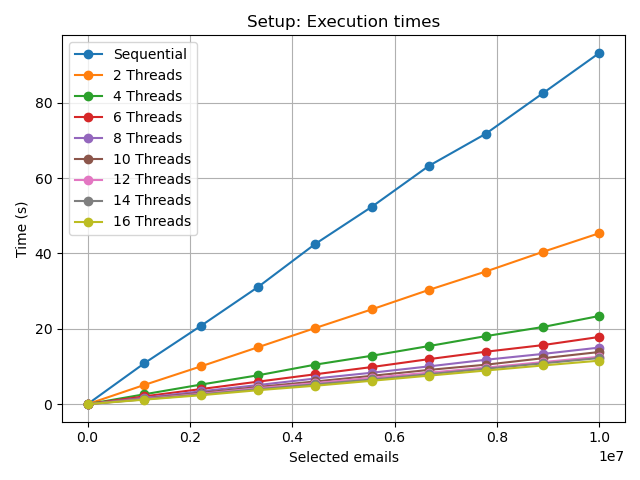
\includegraphics[width=\linewidth]{openmp/005/setup_times}
        \caption{Time setup Omp}\label{fig:005-setup_time_omp}
    \endminipage\hfill
    \minipage{0.49\textwidth}
    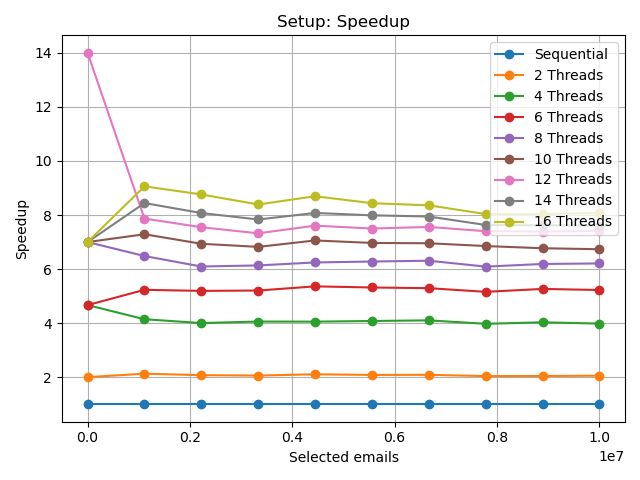
\includegraphics[width=\linewidth]{openmp/005/setup_speedup}
        \caption{Speedup setup Omp}\label{fig:005-setup_speedup_omp}
    \endminipage\hfill
\end{figure}
\begin{figure}[H]
    \centering
    \minipage{0.49\textwidth}
    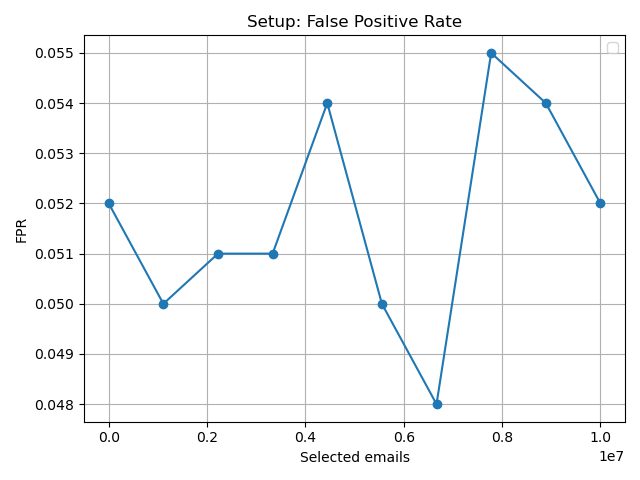
\includegraphics[width=\linewidth]{openmp/005/setup_fpr}
        \caption{FPR setup Omp}\label{fig:005-setup_fpr_omp}
    \endminipage\hfill
\end{figure}

Nell'analisi del tempo di esecuzione e dello speedup, emerge chiaramente come incrementando il numero di processi,
il tempo di esecuzione diminuisce significativamente rispetto alla versione sequenziale, raggiungendo un massimo di 9
con l'utilizzo di 16 processi.
È osservabile che all'aumentare del numero di processi, l'incremento dello speedup presenta una riduzione,
stabilizzandosi al valore di 8.
Per quanto concerne il False Positive Rate, i risultati ottenuti si collocano attorno al valore di FPR del 0,05, cioè
il valore per il quale è stato configurato per il BloomFilter.

\subsubsection{Filter}\label{subsubsec:fpr-005-filter}
\begin{figure}[H]
    \centering
    \minipage{0.49\textwidth}
    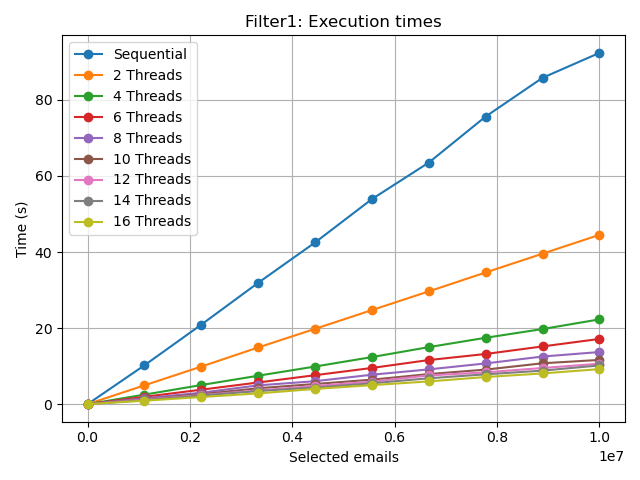
\includegraphics[width=\linewidth]{openmp/005/filter1_times}
        \caption{Time Filter Omp}\label{fig:005-filter_time_omp}
    \endminipage\hfill
    \minipage{0.49\textwidth}
    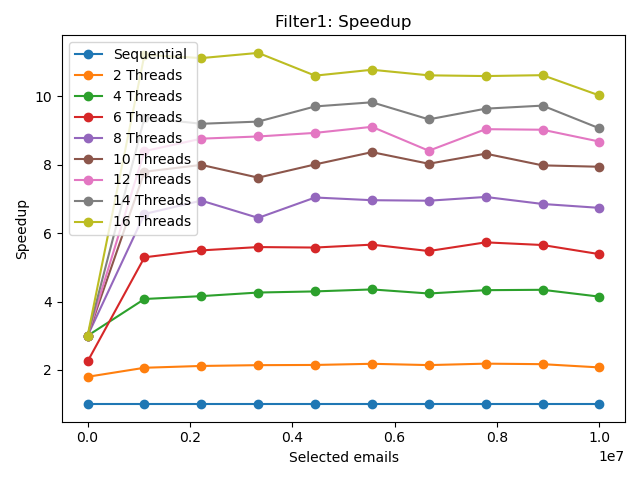
\includegraphics[width=\linewidth]{openmp/005/filter1_speedup}
        \caption{Speedup Filter Omp}\label{fig:005-filter_speedup_omp}
    \endminipage\hfill
\end{figure}
\begin{figure}[H]
    \centering
    \minipage{0.49\textwidth}
    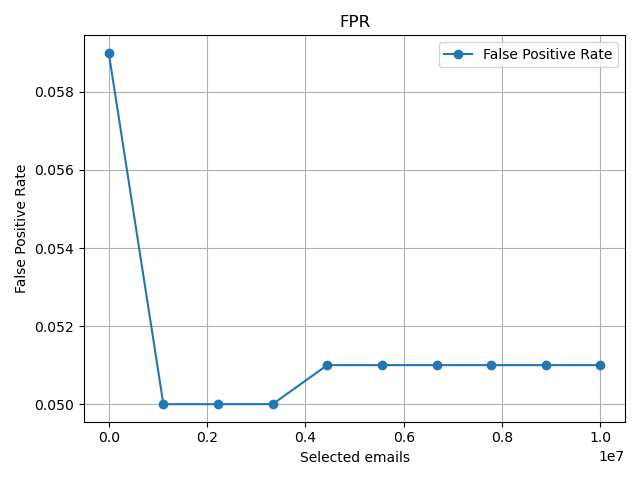
\includegraphics[width=\linewidth]{openmp/005/filter_fpr}
        \caption{FPR Filter Omp}\label{fig:005-filter_fpr_omp}
    \endminipage\hfill
\end{figure}

Analogamente alla fase di setup, nell'incrementare il numero di processi, si osserva una significativa riduzione del
tempo di esecuzione rispetto alla modalità sequenziale, con un picco massimo di 11 utilizzando 16 processi.
In questa circostanza, tuttavia, la diminuzione dello speedup, al variare dei processi, non è altrettanto marcata
rispetto alla fase di setup.
Il valore di FPR raggiunge una sorta di plateau una volta che un numero sufficiente di email è stato raggiunto.

\subsubsection{Confronto Filter}\label{subsubsec:confronto-filter}
Qui vengono esaminate le differenze tra le due versioni implementate del filtro.

\begin{figure}[H]
    \centering
    \minipage{0.49\textwidth}
    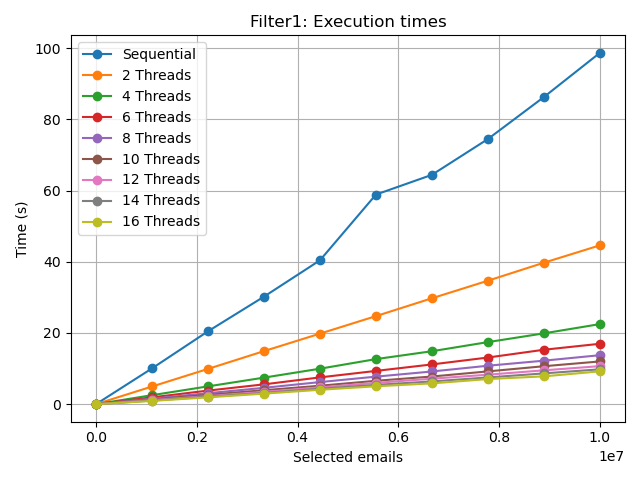
\includegraphics[width=\linewidth]{openmp/filters-005/filter1_times}
        \caption{Time Filter 1}\label{fig:005-filter1_time_omp}
    \endminipage\hfill
    \minipage{0.49\textwidth}
    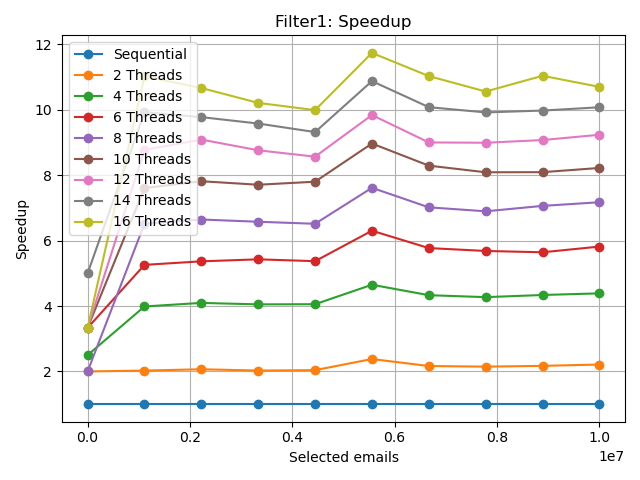
\includegraphics[width=\linewidth]{openmp/filters-005/filter1_speedup}
        \caption{Speedup Filter 1}\label{fig:005-filter1_speedup_omp}
    \endminipage\hfill
\end{figure}
\begin{figure}[H]
    \centering
    \minipage{0.49\textwidth}
    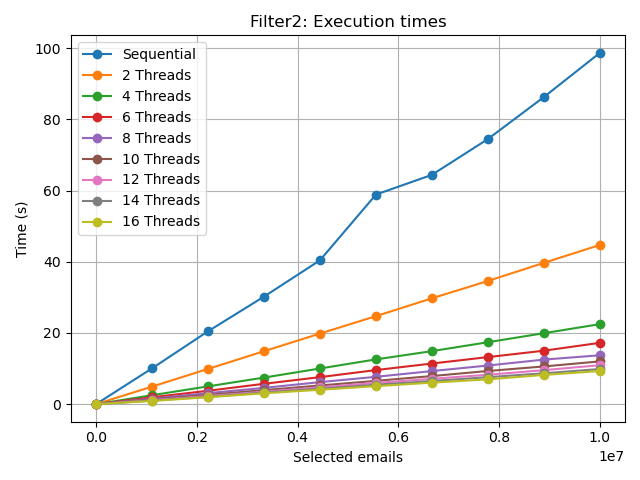
\includegraphics[width=\linewidth]{openmp/filters-005/filter2_times}
        \caption{Time Filter 2}\label{fig:005-filter2_time_omp}
    \endminipage\hfill
    \minipage{0.49\textwidth}
    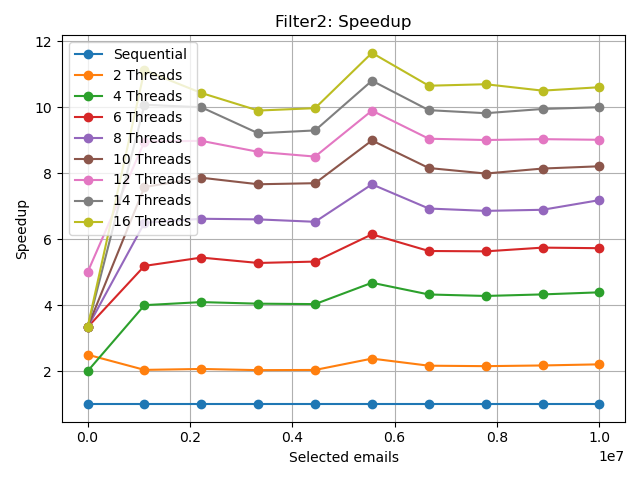
\includegraphics[width=\linewidth]{openmp/filters-005/filter2_speedup}
        \caption{Speedup Filter 2}\label{fig:005-filter2_speedup_omp}
    \endminipage\hfill
\end{figure}

Come evidente, le due versioni del filtro mostrano performance praticamente identiche sia in termini di tempo di
esecuzione che di speedup.
Pertanto, a causa di questa similitudine prestazionale, prenderemo in considerazione la prima implementazione per
le analisi successive.

\subsection{Joblib}\label{subsec:joblib-test}
\subsubsection{Setup}\label{subsubsec:joblib-setup}
\begin{figure}[H]
    \centering
    \minipage{0.49\textwidth}
    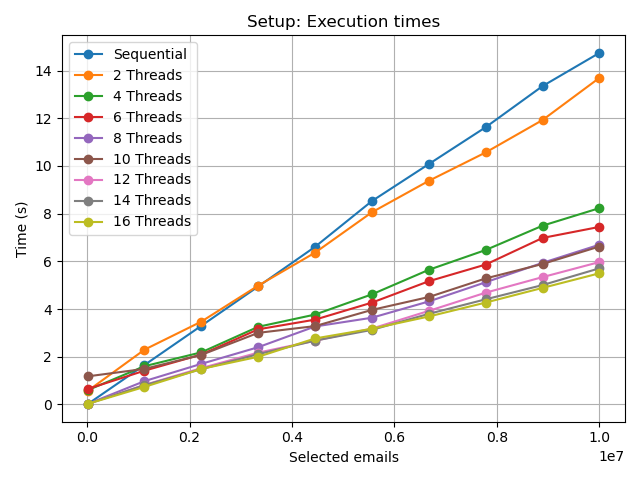
\includegraphics[width=\linewidth]{joblib/005/setup_time_plot}
        \caption{Time setup Joblib}\label{fig:005-setup_time_joblib}
    \endminipage\hfill
    \minipage{0.49\textwidth}
    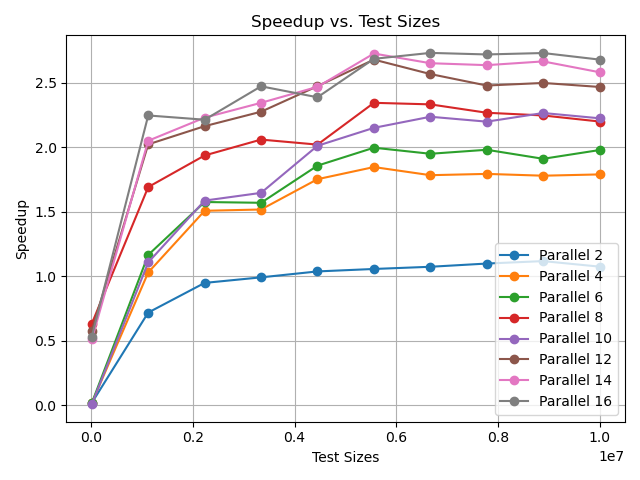
\includegraphics[width=\linewidth]{joblib/005/setup_speedup_plot}
        \caption{Speedup setup Joblib}\label{fig:005-setup_speedup_joblib}
    \endminipage\hfill
\end{figure}
\begin{figure}[H]
    \centering
    \minipage{0.49\textwidth}
    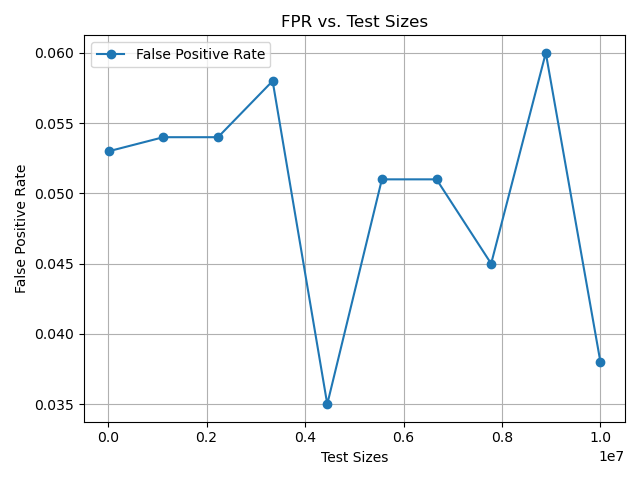
\includegraphics[width=\linewidth]{joblib/005/setup_fpr_plot}
        \caption{FPR setup Joblib}\label{fig:005-setup_fpr_joblib}
    \endminipage\hfill
\end{figure}

I risultati ottenuti nella fase di setup con la versione Joblib evidenziano come l'aumento del numero di processori
conduca a una riduzione del tempo di esecuzione, seppur in maniera meno significativa rispetto alla versione OpenMP\@.
Lo speedup risulta notevole e superiormente performante rispetto alla versione sequenziale una volta che un certo numero
di email è stato raggiunto.
Questo fenomeno è attribuibile al tempo di virtualizzazione dei processi, che in questo caso incide negativamente sul
tempo di esecuzione per un numero ridotto di email.
Il valore massimo di speedup raggiunto si assesta intorno a 2.7.
Anche in questo caso, i valori di FPR (False Positive Rate) si collocano attorno al valore di 0.05.

\subsubsection{Filter}\label{subsubsec:joblib-filter}
\begin{figure}[H]
    \centering
    \minipage{0.49\textwidth}
    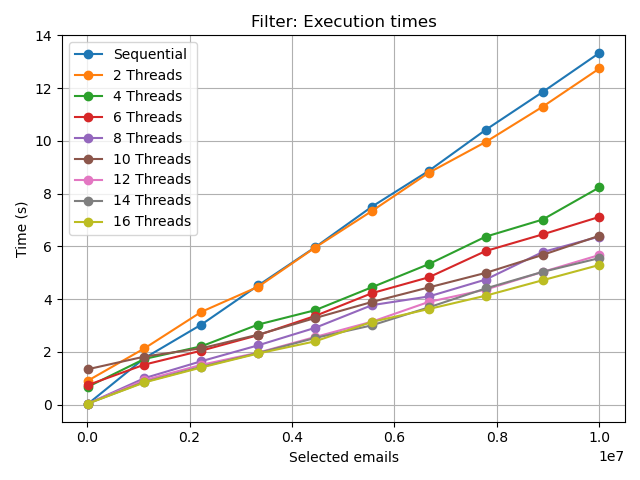
\includegraphics[width=\linewidth]{joblib/005/filter_time_plot}
        \caption{Time Filter Joblib}\label{fig:005-filter_time_joblib}
    \endminipage\hfill
    \minipage{0.49\textwidth}
    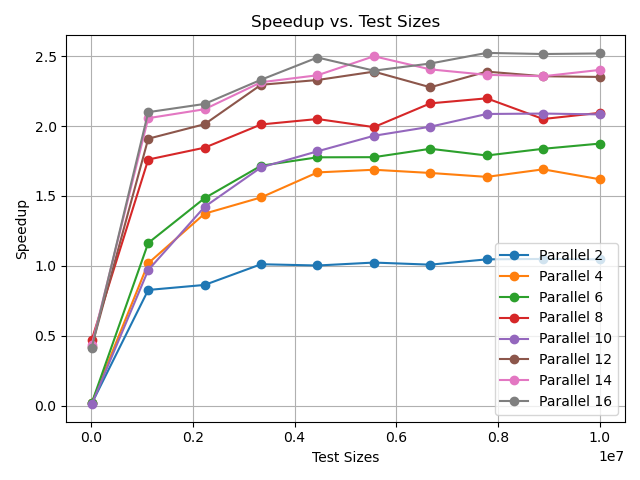
\includegraphics[width=\linewidth]{joblib/005/filter_speedup_plot}
        \caption{Speedup Filter Joblib}\label{fig:005-filter_speedup_joblib}
    \endminipage\hfill
\end{figure}
\begin{figure}[H]
    \centering
    \minipage{0.49\textwidth}
    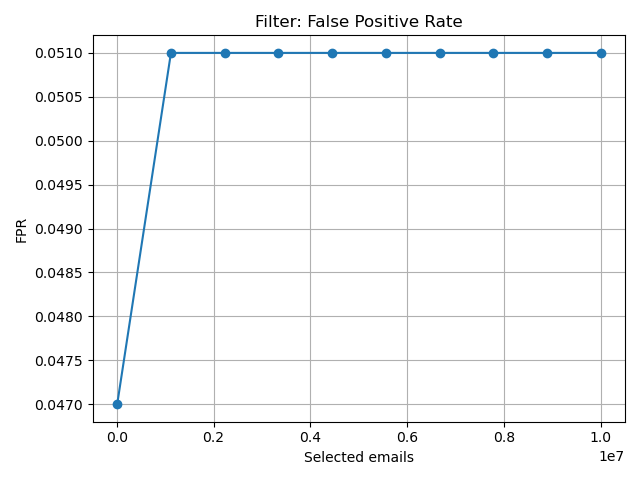
\includegraphics[width=\linewidth]{joblib/005/filter_fpr_plot}
        \caption{FPR Filter Joblib}\label{fig:005-filter_fpr_joblib}
    \endminipage\hfill
\end{figure}

Anche nella fase di filtraggio, come nella fase di setup, l'aumento del numero di processi conduce a una riduzione del
tempo di esecuzione, seppur in maniera meno significativa rispetto alla versione OpenMP\@.
Infatti il valore massimo di speedup raggiunto si assesta intorno a 2.5.
Una volta che un certo numero di email è stato raggiunto, il valore di FPR si stabilizza attorno al valore di 0.05.

\subsubsection{Chunks}\label{subsubsec:005-chunks}
Ora esamineremo la possibilità di eseguire un'operazione di chunking più estesa rispetto al numero di thread disponibili
nella fase di setup per valutare se è possibile migliorare le prestazioni.
I valori di riferimento per i chunk sono 16, 32, 64, 128, 256, 512, 1024, 2048.

\begin{figure}[H]
    \centering
    \minipage{0.49\textwidth}
    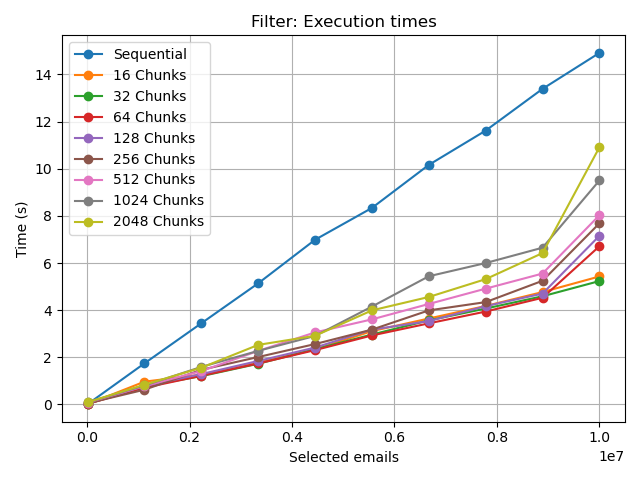
\includegraphics[width=\linewidth]{joblib/005/chunks_time_plot}
        \caption{Times setup Chunks}\label{fig:005-chunks_time}
    \endminipage\hfill
    \minipage{0.49\textwidth}
    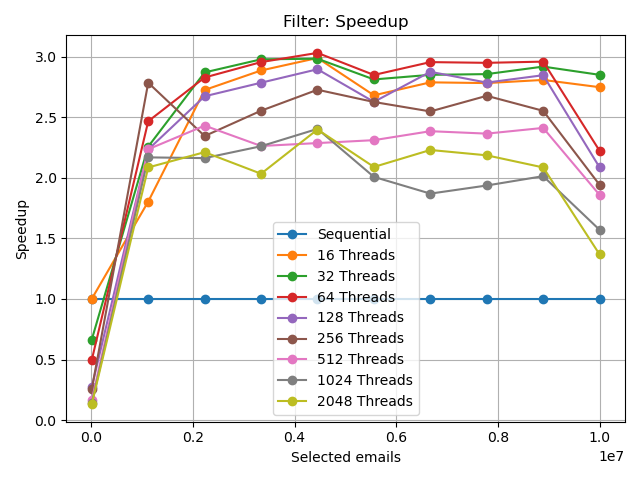
\includegraphics[width=\linewidth]{joblib/005/chunks_speedup_plot}
        \caption{Speedup setup Chunks}\label{fig:005-chunks_speedup}
    \endminipage\hfill
\end{figure}

I risultati ottenuti suggeriscono che l'implementazione dell'operazione di chunking ha portato a miglioramenti
sostanziali nelle performance di speedup.
In particolare, l'aumento del numero di chunk ha contribuito a un notevole miglioramento dello speedup,
raggiungendo un massimo di 3.
Tuttavia, oltre una soglia di 64 chunk, si è verificato un declino nelle performance.

\subsection{Confronto}\label{subsec:confronto}
\subsection{Setup}\label{subsec:confronto-setup}
Nel test di configurazione iniziale, è evidente che la versione sviluppata con OpenMP presenta una performance temporale
inferiore rispetto alla sua controparte.
Al contrario, in termini di speedup, la versione OpenMP supera quella sviluppata con Joblib,
raggiungendo uno speedup massimo di 2.70 nella versione Joblib e 9 nella versione OpenMP,
sfruttando il massimo numero di thread disponibili.

\subsection{Filter}\label{subsec:confronto-filter}
Nel test di filtraggio, è evidente che la versione sviluppata con OpenMP presenta una performance temporale inferiore
rispetto alla sua controparte.
Tuttavia, in termini di speedup, la versione OpenMP supera quella sviluppata con Joblib, raggiungendo un massimo di 11
nella versione OpenMP e 2.5 nella versione Joblib, sfruttando il massimo numero di thread disponibili.
I valori di FPR (False Positive Rate) sono praticamente identici tra le due versioni.





    \section{Conclusioni}\label{sec:conclusioni}
    I risultati ottenuti mostrano che la parallelizzazione delle operazioni di setup e filtraggio del BloomFilter
    consente di ottenere uno speedup significativo in relazione al numero di processori impiegati.
    Specificamente, in termini di tempo, la versione parallelizzata con Joblib è risultata più efficiente rispetto
    alla versione parallelizzata con Omp.
    Viceversa, la versione parallelizzata con Omp ha mostrato un miglioramento più significativo in termini di speedup.
    L'operazione di chunking ha permesso di ottenere uno speedup leggermente migliore rispetto alla versione senza chunking
    per alcuni valori di chunk size.

    \clearpage

    \appendix
    \section{FPR: 0.01}\label{sec:fpr-001}
\subsection{Setup}\label{subsec:setup}
\begin{figure}[H]
    \centering
    \minipage{0.49\textwidth}
    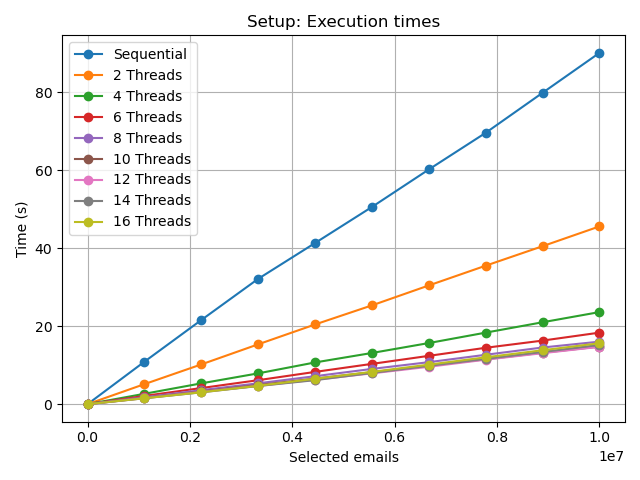
\includegraphics[width=\linewidth]{openmp/001/setup_times}
        \caption{Speedup setup Omp}\label{fig:setup_time_omp}
    \endminipage\hfill
    \minipage{0.49\textwidth}
    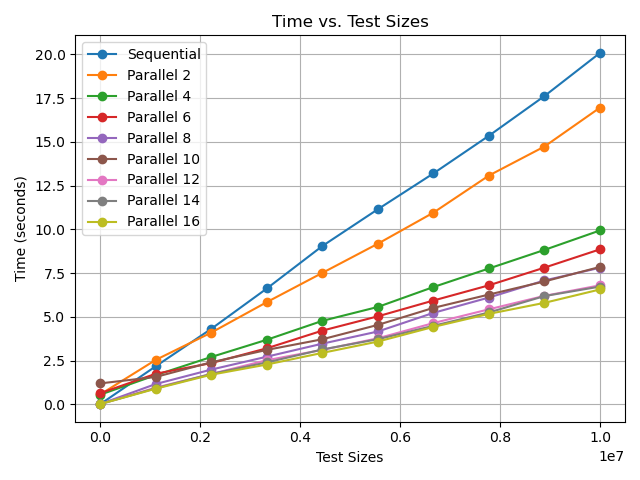
\includegraphics[width=\linewidth]{joblib/001/setup_time_plot}
        \caption{Speedup setup Joblib}\label{fig:setup_time_joblib}
    \endminipage\hfill
\end{figure}
\begin{figure}[H]
    \centering
    \minipage{0.49\textwidth}
    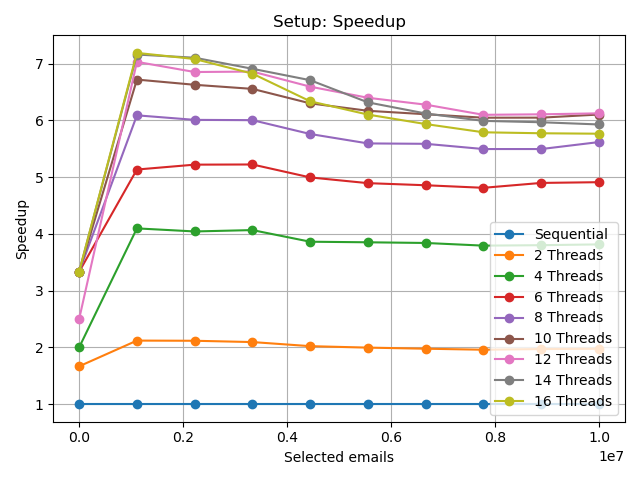
\includegraphics[width=\linewidth]{openmp/001/setup_speedup}
        \caption{Speedup setup Omp}\label{fig:setup_speedup_omp}
    \endminipage\hfill
    \minipage{0.49\textwidth}
    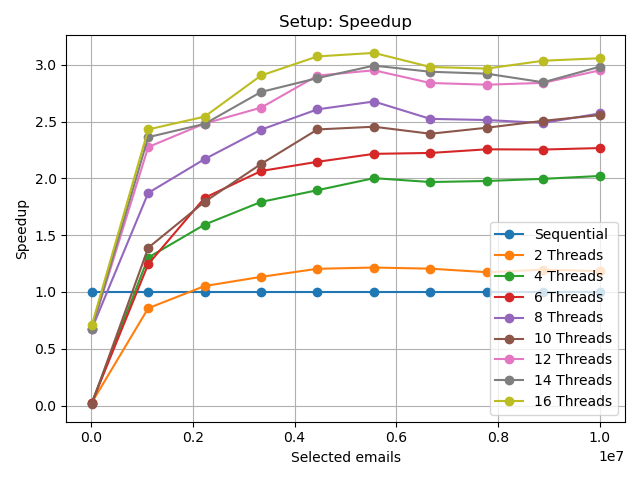
\includegraphics[width=\linewidth]{joblib/001/setup_speedup_plot}
        \caption{Speedup setup Joblib}\label{fig:setup_speedup_joblib}
    \endminipage\hfill
\end{figure}
\begin{figure}[H]
    \centering
    \minipage{0.49\textwidth}
    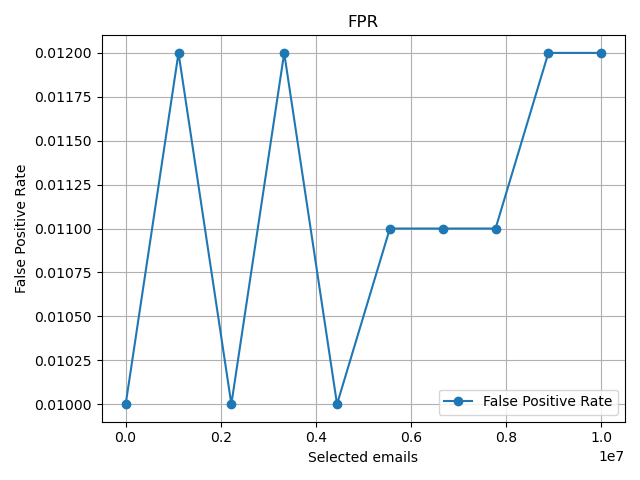
\includegraphics[width=\linewidth]{openmp/001/setup_fpr}
        \caption{Speedup setup Omp}\label{fig:setup_fpr_omp}
    \endminipage\hfill
    \minipage{0.49\textwidth}
    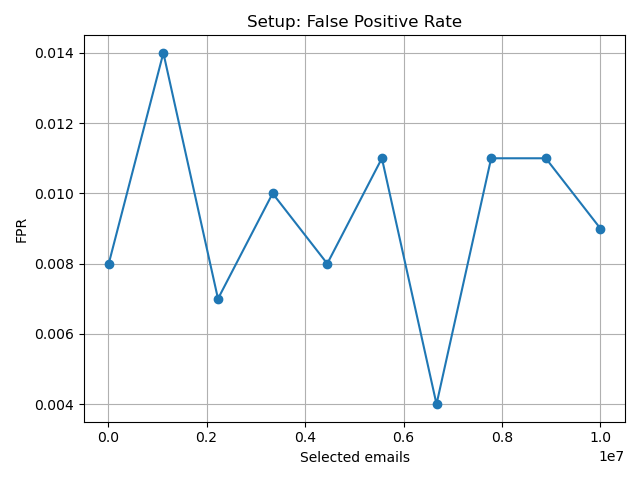
\includegraphics[width=\linewidth]{joblib/001/setup_fpr_plot}
        \caption{Speedup setup Joblib}\label{fig:setup_fpr_joblib}
    \endminipage\hfill
\end{figure}

\subsection{Filter}\label{subsec:filter}
\begin{figure}[H]
    \centering
    \minipage{0.49\textwidth}
    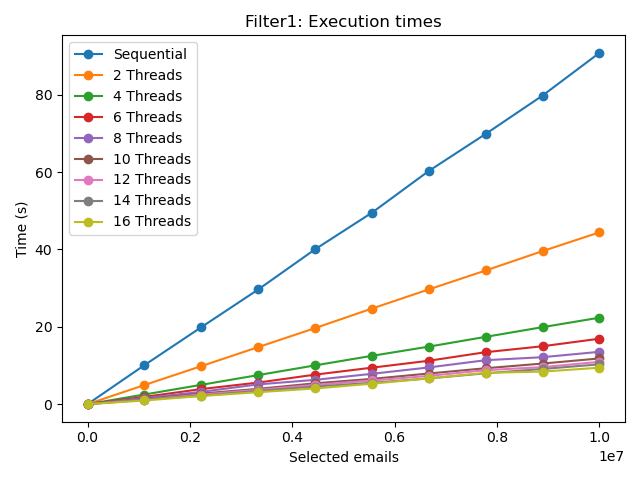
\includegraphics[width=\linewidth]{openmp/001/filter1_times}
        \caption{Times filter Omp}\label{fig:filter_time_omp}
    \endminipage\hfill
    \minipage{0.49\textwidth}
    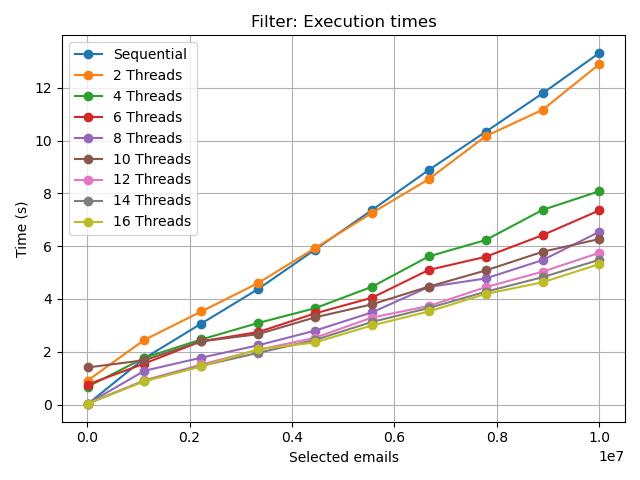
\includegraphics[width=\linewidth]{joblib/001/filter_time_plot}
        \caption{Times filter Joblib}\label{fig:filter_time_joblib}
    \endminipage\hfill
\end{figure}
\begin{figure}[H]
    \centering
    \minipage{0.49\textwidth}
    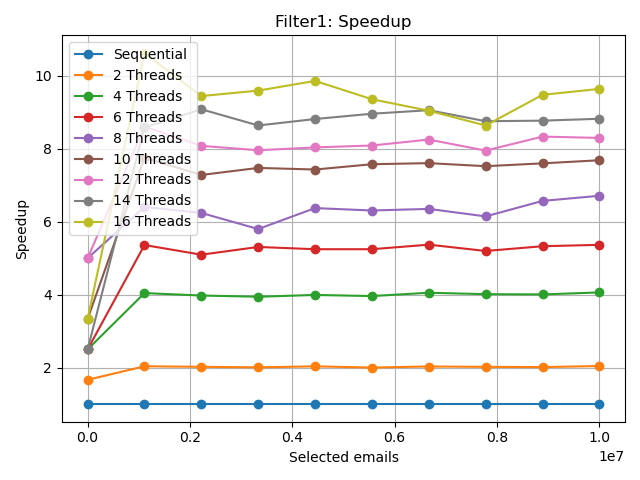
\includegraphics[width=\linewidth]{openmp/001/filter1_speedup}
        \caption{Speedup filter Omp}\label{fig:filter_speedup_omp}
    \endminipage\hfill
    \minipage{0.49\textwidth}
    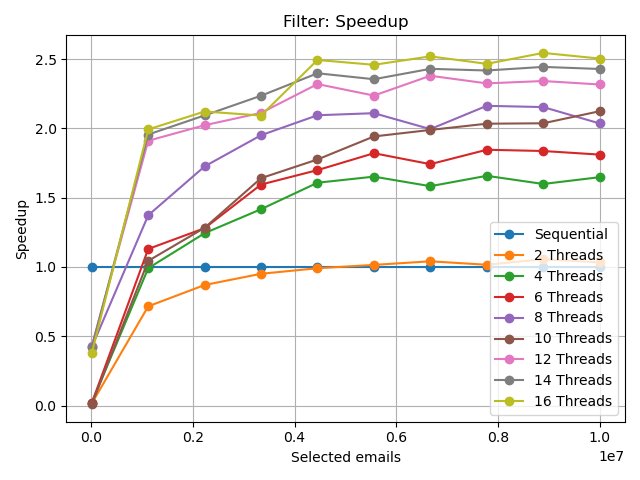
\includegraphics[width=\linewidth]{joblib/001/filter_speedup_plot}
        \caption{Speedup filter Joblib}\label{fig:filter_speedup_joblib}
    \endminipage\hfill
\end{figure}
\begin{figure}[H]
    \centering
    \minipage{0.49\textwidth}
    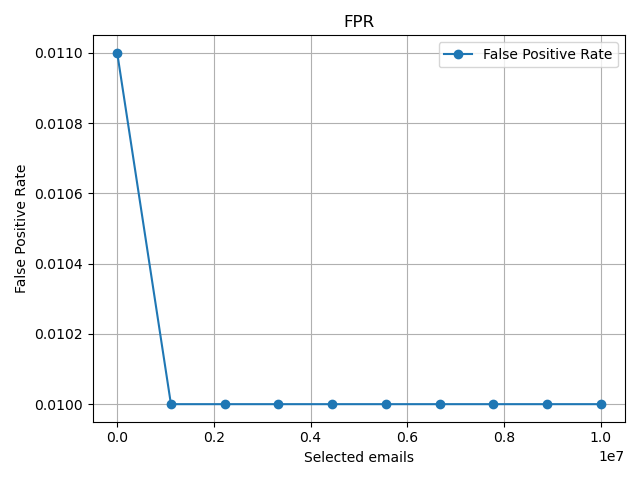
\includegraphics[width=\linewidth]{openmp/001/filter_fpr}
        \caption{FPR filter Omp}\label{fig:filter_fpr_omp}
    \endminipage\hfill
    \minipage{0.49\textwidth}
    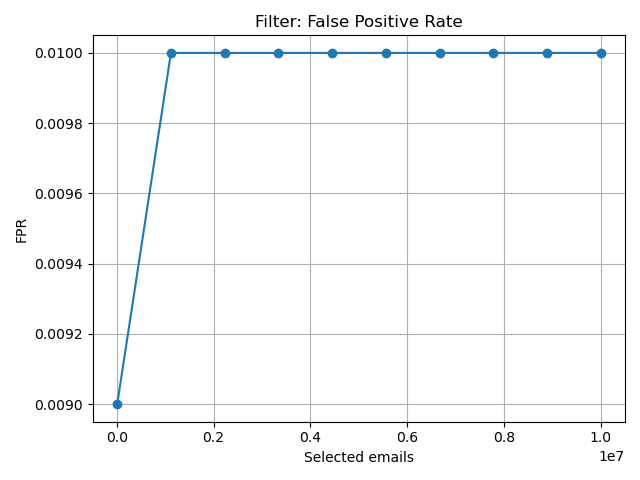
\includegraphics[width=\linewidth]{joblib/001/filter_fpr_plot}
        \caption{FPR filter Joblib}\label{fig:filter_fpr_joblib}
    \endminipage\hfill
\end{figure}

\subsection{Chunks}\label{subsec:chunks}
\begin{figure}[H]
    \centering
    \minipage{0.49\textwidth}
    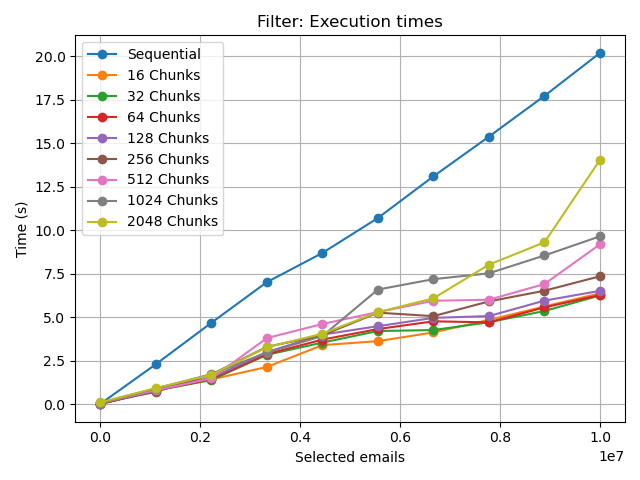
\includegraphics[width=\linewidth]{joblib/001/chunks_time_plot}
        \caption{Times chunks Joblib}\label{fig:chunks_time_joblib}
    \endminipage\hfill
    \minipage{0.49\textwidth}
    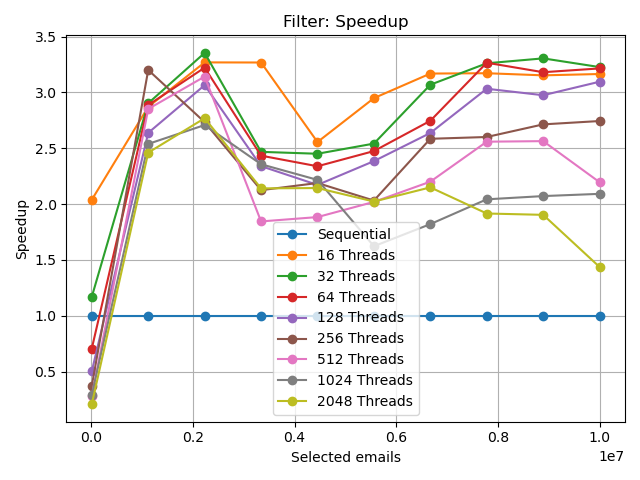
\includegraphics[width=\linewidth]{joblib/001/chunks_speedup_plot}
        \caption{Speedup chunks Joblib}\label{fig:chunks_speedup_joblib}
    \endminipage\hfill
\end{figure}

\section{FPR: 0.10}\label{sec:fpr-010}
\subsection{Setup}\label{subsec:fpr-010-setup}
\begin{figure}[H]
    \centering
    \minipage{0.49\textwidth}
    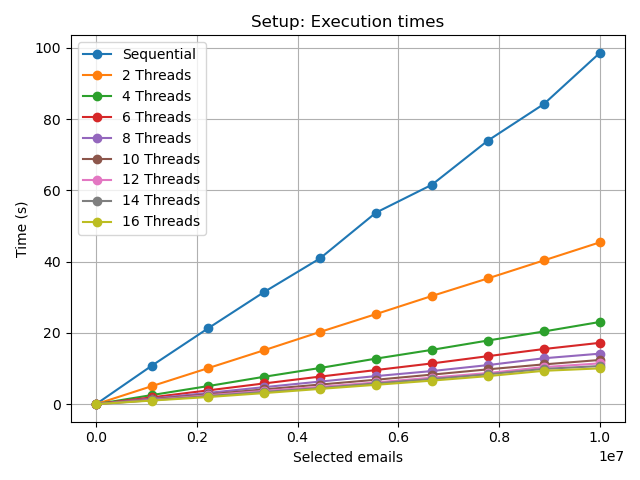
\includegraphics[width=\linewidth]{openmp/010/setup_times}
        \caption{Time setup Omp}\label{fig:010-setup_time_omp}
    \endminipage\hfill
    \minipage{0.49\textwidth}
    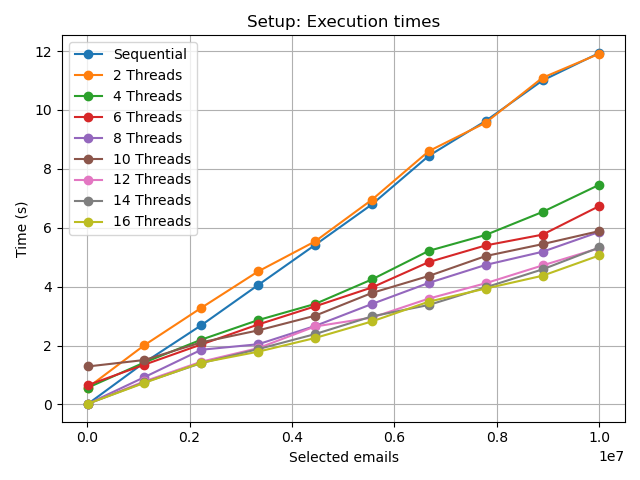
\includegraphics[width=\linewidth]{joblib/010/setup_time_plot}
        \caption{Time setup Joblib}\label{fig:010setup_time_joblib}
    \endminipage\hfill
\end{figure}
\begin{figure}[H]
    \centering
    \minipage{0.49\textwidth}
    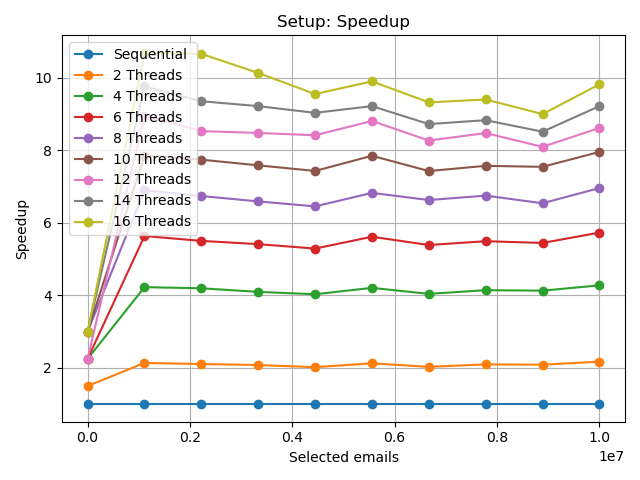
\includegraphics[width=\linewidth]{openmp/010/setup_speedup}
        \caption{Speedup setup Omp}\label{fig:010-setup_speedup_omp}
    \endminipage\hfill
    \minipage{0.49\textwidth}
    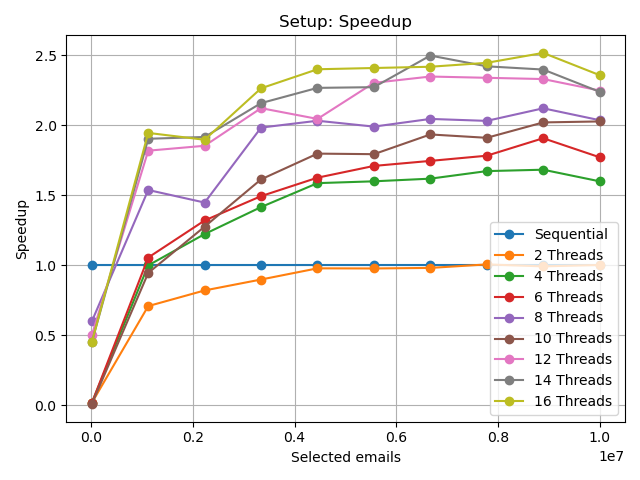
\includegraphics[width=\linewidth]{joblib/010/setup_speedup_plot}
        \caption{Speedup setup Joblib}\label{fig:010-setup_speedup_joblib}
    \endminipage\hfill
\end{figure}
\begin{figure}[H]
    \centering
    \minipage{0.49\textwidth}
    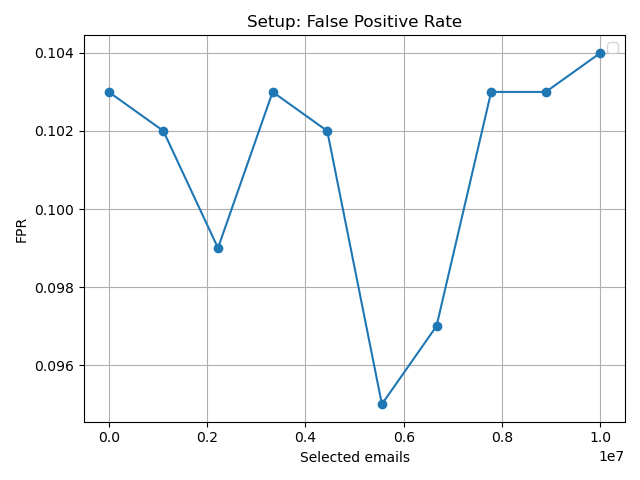
\includegraphics[width=\linewidth]{openmp/010/setup_fpr}
        \caption{FPR setup Omp}\label{fig:010-setup_fpr_omp}
    \endminipage\hfill
    \minipage{0.49\textwidth}
    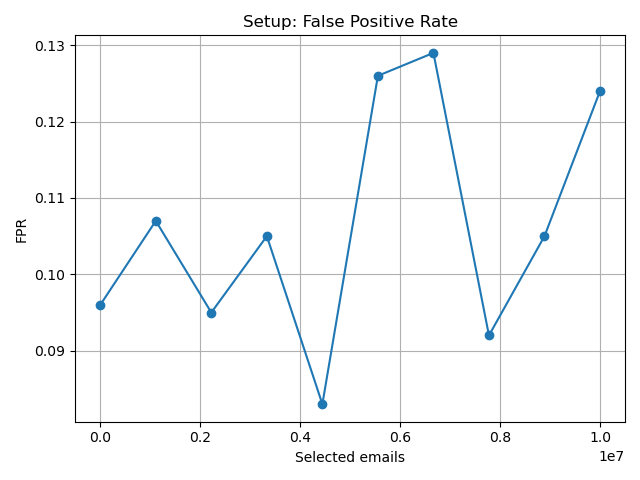
\includegraphics[width=\linewidth]{joblib/010/setup_fpr_plot}
        \caption{FPR setup Joblib}\label{fig:010-setup_fpr_joblib}
    \endminipage\hfill
\end{figure}
\subsection{Filter}\label{subsec:fpr-010-filter}
\begin{figure}[H]
    \centering
    \minipage{0.49\textwidth}
    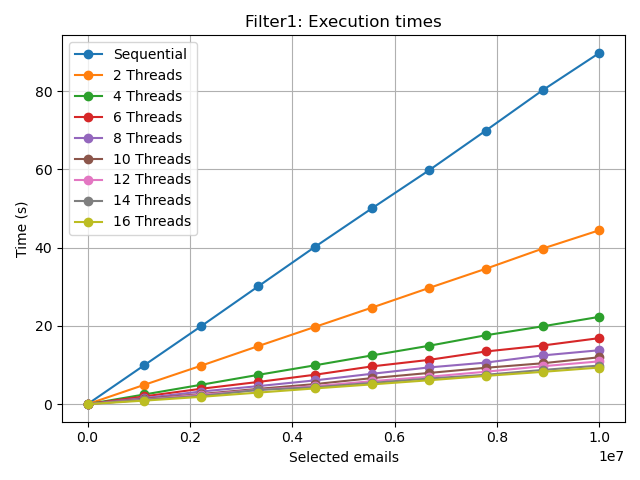
\includegraphics[width=\linewidth]{openmp/010/filter1_times}
        \caption{Time setup Omp}\label{fig:010-filter_time_omp}
    \endminipage\hfill
    \minipage{0.49\textwidth}
    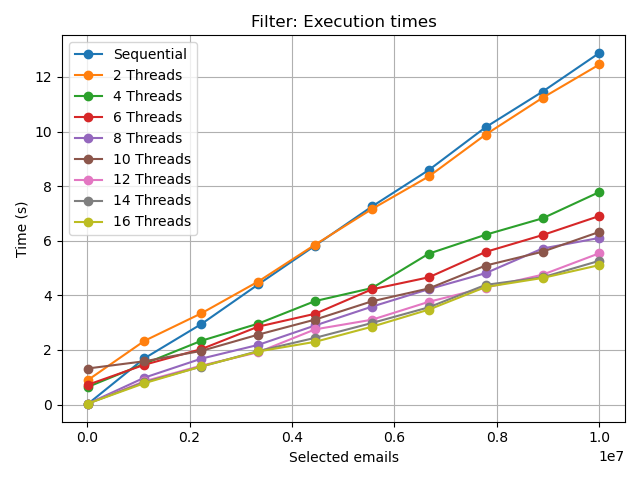
\includegraphics[width=\linewidth]{joblib/010/filter_time_plot}
        \caption{Speedup setup Joblib}\label{fig:010-filter_time_joblib}
    \endminipage\hfill
\end{figure}
\begin{figure}[H]
    \centering
    \minipage{0.49\textwidth}
    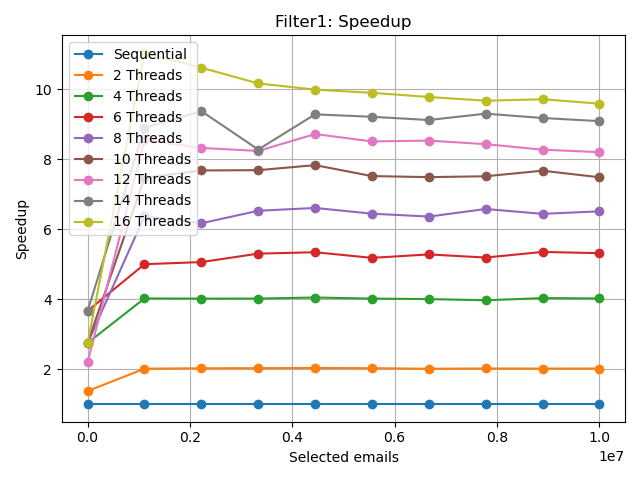
\includegraphics[width=\linewidth]{openmp/010/filter1_speedup}
        \caption{Speedup setup Omp}\label{fig:010-filter_speedup_omp}
    \endminipage\hfill
    \minipage{0.49\textwidth}
    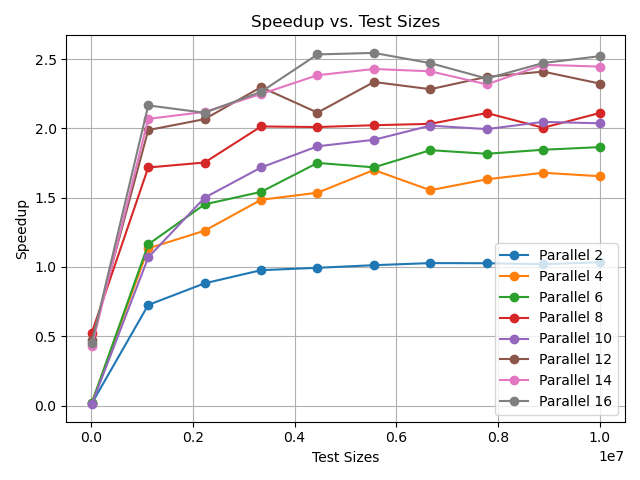
\includegraphics[width=\linewidth]{joblib/010/filter_speedup_plot}
        \caption{Speedup setup Joblib}\label{fig:010-filter_speedup_joblib}
    \endminipage\hfill
\end{figure}
\begin{figure}[H]
    \centering
    \minipage{0.49\textwidth}
    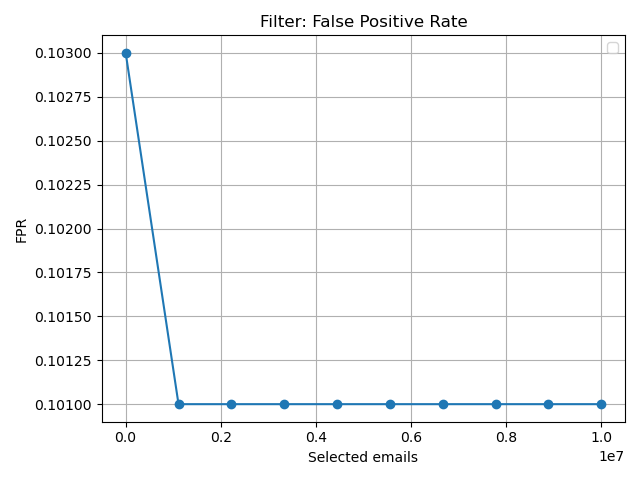
\includegraphics[width=\linewidth]{openmp/010/filter_fpr}
        \caption{FPR Filter Omp}\label{fig:010-filter_fpr_omp}
    \endminipage\hfill
    \minipage{0.49\textwidth}
    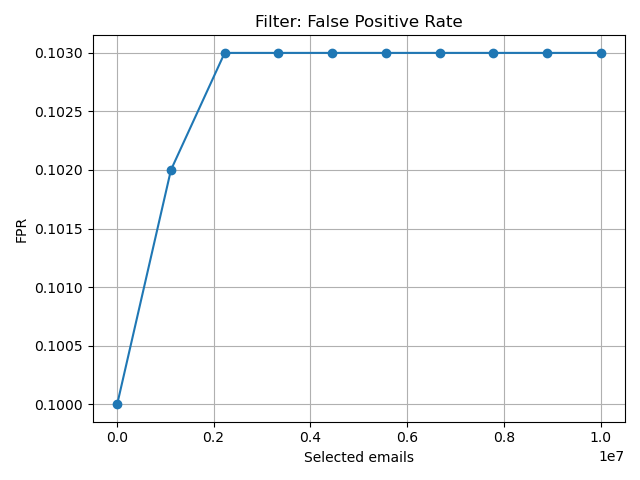
\includegraphics[width=\linewidth]{joblib/010/filter_fpr_plot}
        \caption{FPR Filter Joblib}\label{fig:010-filter_fpr_joblib}
    \endminipage\hfill
\end{figure}
\subsection{Chunks}\label{subsec:010-chunks}
\begin{figure}[H]
    \centering
    \minipage{0.49\textwidth}
    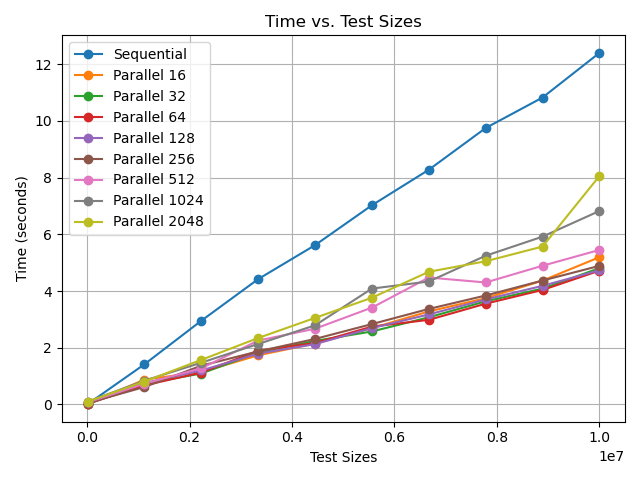
\includegraphics[width=\linewidth]{joblib/010/chunks_time_plot}
        \caption{Times setup Chunk}\label{fig:010-chunks_time}
    \endminipage\hfill
    \minipage{0.49\textwidth}
    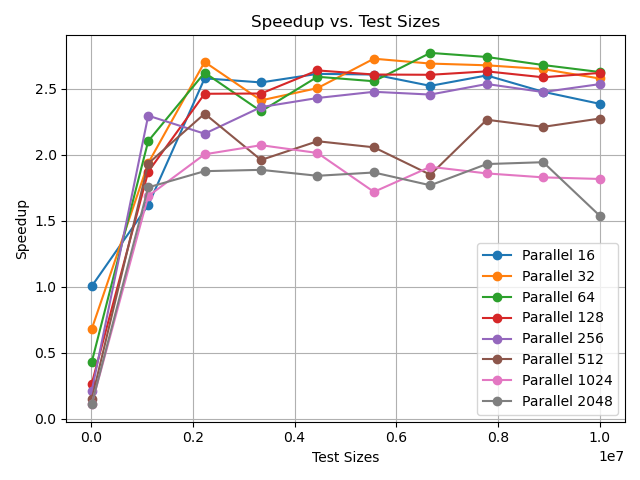
\includegraphics[width=\linewidth]{joblib/010/chunks_speedup_plot}
        \caption{Speedup setup Chunk}\label{fig:010-chunks_speedup}
    \endminipage\hfill
\end{figure}


\end{document}